\section{Programação e lógica em LADDER}


\begin{frame}{Norma IEC 61131-3}
	\begin{block}{Introdução}
		A \textbf{norma IEC 61131} define os padrões de operação dos CLPs, inclusive as linguagens de programação às quais devem ser capazes de operar (item 3). São elas:
		\begin{itemize}
			\item Texto Estruturado (ST)
			\item Lista de Instruções (IL)
			\item Diagrama Ladder (LD)
			\item Diagramas de Blocos Funcionais (FBD)
			\item Funções Gráficas de Sequenciamento (SFC)
			\item Funções Gráficas Contínuas (CFC)
		\end{itemize}
	
		Além disso, essa norma também permite a chamada de \textbf{outras linguagens} de programação, além de \textbf{diferentes abordagens} para a construção de um projeto de CLP.
	\end{block}
\end{frame}


\begin{frame}{Norma IEC 61131-3}
	\begin{block}{Texto Estruturado - \textit{Structured Text}}
		\begin{itemize}
			\item É uma linguagem baseada em Pascal, e é similar à algumas linguagens de texto menos modernas.
			\item É uma ferramenta poderosa, que pode ser utilizada para a execução de \textbf{algoritmos matemáticos complexos}.
		\end{itemize}
	\end{block}

	\centering
	
	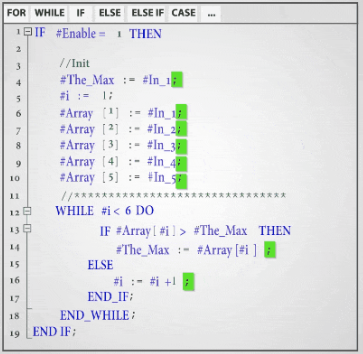
\includegraphics[height=0.6\textheight]{Figuras/Ch10/fig1}
	
\end{frame}


\begin{frame}{Norma IEC 61131-3}
	\begin{block}{Lista de Instruções - \textit{Instruction List}}
		\begin{itemize}
			\item É uma linguagem muito similar à \textit{Assembly}.
			\item É \textbf{rápida} e produz um programa \textbf{compacto}, porém é \textbf{muito difícil} de programar.
		\end{itemize}
	\end{block}

	\centering
	
	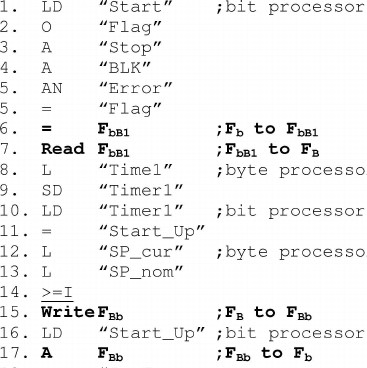
\includegraphics[height=0.6\textheight]{Figuras/Ch10/fig2}
\end{frame}


\begin{frame}{Norma IEC 61131-3}
	\begin{block}{Diagrama Ladder - \textit{Ladder Diagram}}
		\begin{itemize}
			\item Baseia-se na lógica de \textbf{diagramas elétricos}.
			\item É \textbf{fácil} de seguir e entender.
			\item Não acomoda algumas \textbf{funções complexas}.
		\end{itemize}
	\end{block}

	\centering

	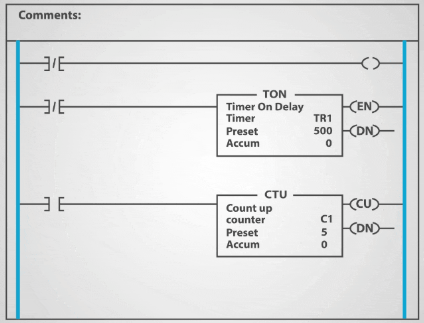
\includegraphics[height=0.6\textheight]{Figuras/Ch10/fig3}
	
\end{frame}


\begin{frame}{Norma IEC 61131-3}
	\begin{block}{Diagramas de Blocos Funcionais - \textit{Function Block Diagram}}
		\begin{itemize}
			\item Esta linguagem de programação se organiza em blocos.
			\item A programação é \textbf{altamente modular}, já que vários blocos podem se unir em \textbf{um só}.
			\item É \textbf{muito difícil} de encontrar erros.
		\end{itemize}
	\end{block}

	\centering
	
	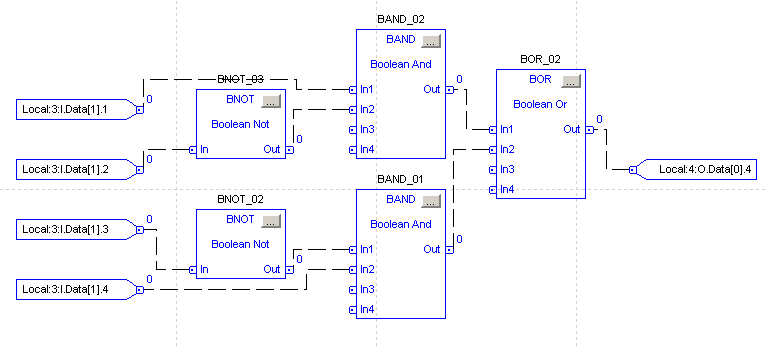
\includegraphics[height=0.6\textheight]{Figuras/Ch10/fig4}
\end{frame}


\begin{frame}{Norma IEC 61131-3}
	\begin{block}{Funções Gráficas de Sequenciamento - \textit{Sequential Function Chart}}
		\begin{itemize}
			\item Baseia-se na ideia de um \textbf{fluxograma}, seguindo \textbf{passos} e \textbf{transições}.
			\item É \textbf{fácil} de programar e de encontrar erros.
			\item Não se aplica a todos os processos.
		\end{itemize}
	\end{block}

	\centering
	
	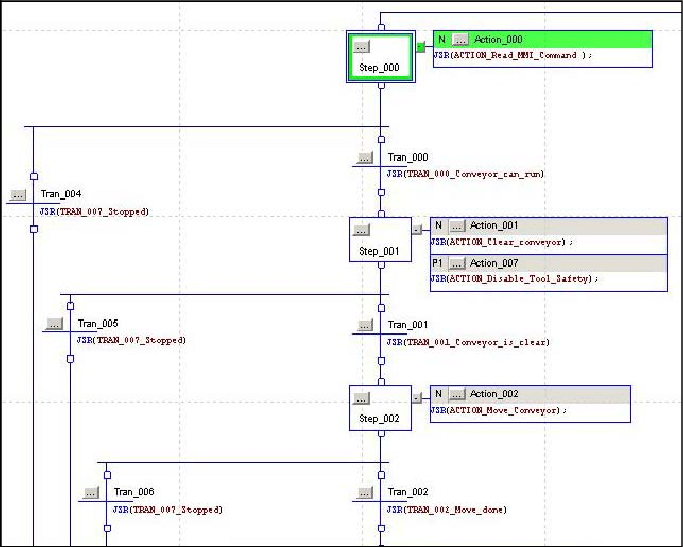
\includegraphics[height=0.6\textheight]{Figuras/Ch10/fig5}
\end{frame}


\begin{frame}{Norma IEC 61131-3}
	\begin{block}{Funções Gráficas Contínuas - \textit{Continuous Function Chart}}
		\begin{itemize}
			\item É similar ao SFC, porém para processos \textbf{contínuos}.
		\end{itemize}
	\end{block}

	\centering
	
	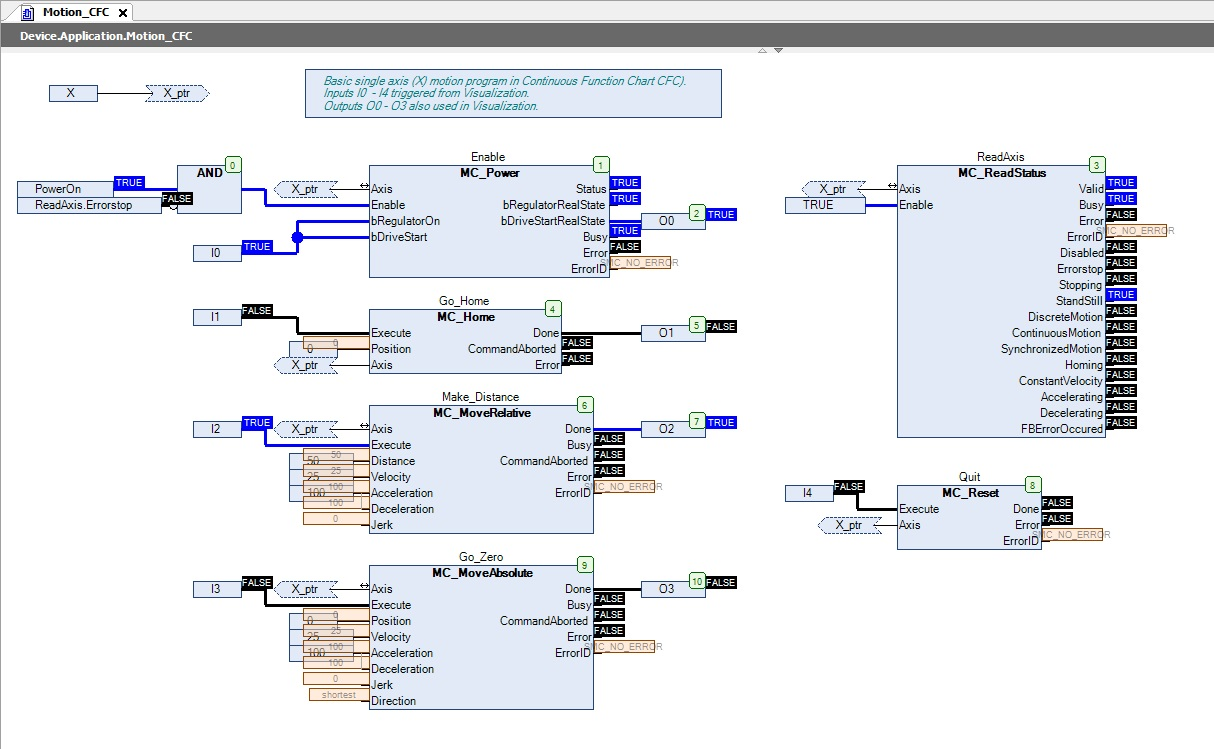
\includegraphics[height=0.7\textheight]{Figuras/Ch10/fig6}
\end{frame}


\begin{frame}{Diagrama Ladder}
	\begin{block}{Introdução}
		\begin{itemize}
			\item Na linguagem \textit{Ladder} (``escada'', em português), cada ``degrau'' é uma \textbf{regra}, dividida, geralmente, em \textbf{duas partes}:
		\end{itemize}
	\end{block}

	\vspace{0.5cm}

	\centering

	\begin{tikzpicture}[circuit plc ladder, thick,x=\ladderskip,y=\ladderskip]
		% drawing
		\draw[blue,thick,dashed] (-0.5,0.7) -- ++(2.5,0) -- ++(0,-1.9) -- ++(-2.5,0);
%		\draw[red,thick,dashed] (-0.5,0.7) -- ++(2.5,0) -- ++(0,-1.9) -- ++(-2.5,0);
		
		\draw (0,0) to[contact NO={info={a}}] ++(2,0) to[coil={info={b}}] ++(2,0) coordinate(laddertopright);
		\ladderrungend{2}
		
		\powerrails
		
	\end{tikzpicture}
	
	\begin{block}{Parte esquerda}
		Na \textbf{parte esquerda} do degrau há a \textbf{condição} para que a outra parte se ative.
	\end{block}
\end{frame}


\begin{frame}{Diagrama Ladder}
	\begin{block}{Parte direita}
		Na \textbf{parte direita} do degrau fica o \textbf{comando} que deve ser ativado.
	\end{block}
	
	\vspace{0.5cm}
	
	\centering
	
	\begin{tikzpicture}[circuit plc ladder, thick,x=\ladderskip,y=\ladderskip]
		% drawing
%		\draw[blue,thick,dashed] (-0.5,0.7) -- ++(2.5,0) -- ++(0,-1.9) -- ++(-2.5,0);
		\draw[red,thick,dashed] (4.5,0.7) -- ++(-2.5,0) -- ++(0,-1.9) -- ++(2.5,0);
		
		\draw (0,0) to[contact NO={info={a}}] ++(2,0) to[coil={info={b}}] ++(2,0) coordinate(laddertopright);
		\ladderrungend{2}
		
		\powerrails
	
	\end{tikzpicture}
	
	\begin{block}{Ordem de leitura}
		Sendo assim, cada degrau deve ser lido da \textbf{esquerda para a direita}, como uma instrução, ou, regra.
	\end{block}
\end{frame}


\begin{frame}{Diagrama Ladder}
	\begin{block}{Tipos de comandos básicos}
		\begin{itemize}
			\item Como o Ladder é baseado em \textbf{circuitos elétricos}, grande parte de seus comandos são herdados de lá.
		\end{itemize}
	\end{block}

	\vspace{0.5cm}
	
	\centering
	
	\begin{tikzpicture}[circuit plc ladder, thick,x=\ladderskip,y=\ladderskip]
	
		\draw (0,0) to[contact NO] node[below=10pt] {Contato NA} ++(1,0);
		\draw (4,0) to[var contact NC] node[below=10pt] {Contato NF} ++(1,0);
		\draw (0,-2) to[coil] node[below=10pt] {Bobina NA} ++(1,0);
		\draw (4,-2) to[var coil NA] node[below=10pt] {Bobina NF} ++(1,0);
	
	\end{tikzpicture}
\end{frame}


\begin{frame}{Diagrama Ladder}
	\begin{block}{Tipos de lógica básica}
		\begin{itemize}
			\item É possível fazer todas as lógicas dos diagramas elétricos aqui, também.
		\end{itemize}
	\end{block}
	
	\vspace{0.5cm}
	
	\centering
	
	\begin{tikzpicture}[circuit plc ladder, thick,x=\ladderskip,y=\ladderskip]
	
		\draw (0,0) 
		to[contact NO={info={a}}] ++(2,0) coordinate(laddercoil) -- ++(2,0) 
		to[coil={info={c}}] ++(2,0) coordinate(laddertopright);
		\draw (0,-1) 
		to[contact NO={info={b}}] ++(2,0) -- (laddercoil);
		\ladderrungend{2.5}
		
		\powerrails
	\end{tikzpicture}
	
	\begin{block}{Lógica OU}
		\[ a+b=c \]
	\end{block}
\end{frame}


\begin{frame}{Diagrama Ladder}
	\begin{block}{Lógica E}
		\[ a\cdot b=c \]
	\end{block}
	
	\vspace{0.5cm}
	
	\centering
	
	\begin{tikzpicture}[circuit plc ladder, thick,x=\ladderskip,y=\ladderskip]
	
	\draw (0,0) 
	to[contact NO={info={a}}] ++(1.5,0) 
	to[contact NO={info={b}}] ++(1.5,0) -- ++(2,0) 
	to[coil={info={c}}] ++(2,0) coordinate(laddertopright);
	\ladderrungend{2}
	
	\powerrails
	\end{tikzpicture}
\end{frame}


\begin{frame}{Diagrama Ladder}
	\begin{block}{Revisão}
		01. Escreva as seguintes expressões em Ladder:
		
		\smallskip
		
		(a) \[ a\cdot \notted{b}=c \]
		(b) \[ a\cdot b + c = d \]
		(c) \[ (a+b)\cdot(\notted{c}+d)=e \]
		(d) \[ a\cdot(b+c)=d+e \]
	\end{block}
\end{frame}


\begin{frame}{Diagrama Ladder}
	\begin{block}{Saídas}
		\begin{itemize}
			\item As saídas, em Ladder, ao contrário das entradas, são \textbf{todas acionadas da mesma forma, independentemente de estarem em série ou em paralelo}.
		\end{itemize}
	\end{block}

	\vspace{1cm}

	\begin{minipage}{0.48\linewidth}
		\centering
		\begin{tikzpicture}[circuit plc ladder, thick,x=0.8\ladderskip,y=0.8\ladderskip]
		
		\draw (0,0) 
		to[contact NO={info={a}}] ++(1,0) -- ++(1.5,0) coordinate(laddercoil)
		to[coil={info={b}}] ++(1.5,0) coordinate(laddertopright);
		\draw (laddercoil) -- ++(0,-1) 
		to[coil={info={c}}] ++(1.5,0);
		\ladderrungend{2}
		
		\powerrails
		\end{tikzpicture}
		\tikzmark{p1}
	\end{minipage}
	\hfill
	\begin{minipage}{0.48\linewidth}
		\centering
		\begin{tikzpicture}[circuit plc ladder, thick,x=0.8\ladderskip,y=0.8\ladderskip]
		
		\draw (0,0) 
		to[contact NO={info={a}}] ++(1,0) -- ++(0.5,0) 
		to[coil={info={b}}] ++(1,0)
		to[coil={info={c}}] ++(1,0) coordinate(laddertopright);
		\ladderrungend{1.2}
		
		\powerrails
		\end{tikzpicture}
	\end{minipage}

	\begin{tikzpicture}[remember picture, overlay]
		\draw ($ (p1)+(0.9,1) $) node[] {\Huge $ = $};
	\end{tikzpicture}
\end{frame}


\begin{frame}{Selos}
	\begin{block}{Analogia a circuitos}
		\begin{itemize}
			\item Em Ladder, assim como em circuitos clássicos, podemos realizar o \textbf{selo} utilizando uma bobina e alguns contatos.
			\item Essa bobina pode ser real, ou não.
		\end{itemize}
	\end{block}
	
	\vspace{0.5cm}
	
	\centering
	
	\begin{tikzpicture}[circuit plc ladder, thick,x=1\ladderskip,y=01\ladderskip]
	
	\draw (0,0) 
	to[contact NO={info={a}}] ++(1.5,0) coordinate(laddercoil)
	to[contact NC={info={b}}] ++(2,0) -- ++(1,0)
	to[coil={info={c}}] ++(2,0) coordinate(laddertopright);
	\draw (0,-1)
	to[contact NO={info={c}}] ++ (1.5,0) -- (laddercoil);
	\ladderrungend{2.5}
	
	\powerrails
	\end{tikzpicture}
\end{frame}


\begin{frame}{Selos}
	\begin{minipage}{0.38\linewidth}
		\centering
		
		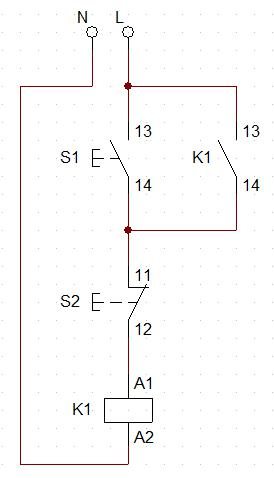
\includegraphics[height=0.8\textheight]{Figuras/Ch10/fig8n2}
	\end{minipage}
	\hfill
	\begin{minipage}{0.6\linewidth}
		\centering
		
		\begin{tikzpicture}[circuit plc ladder, thick,x=1\ladderskip,y=01\ladderskip]
		
		\draw (0,0) 
		to[contact NO={info={a}}] ++(1,0) coordinate(laddercoil)
		to[contact NC={info={b}}] ++(1.5,0) -- ++(0.5,0)
		to[coil={info={c}}] ++(2,0) coordinate(laddertopright);
		\draw (0,-1)
		to[contact NO={info={c}}] ++ (1,0) -- (laddercoil);
		\ladderrungend{2.1}
		
		\powerrails[0.4]
		\end{tikzpicture}
	\end{minipage}

	\bigskip

	\centering

	Comparação entre o circuito original e seu análogo em Ladder
\end{frame}


\begin{frame}{Selos}
	\begin{block}{Latch}
		\begin{itemize}
			\item Em Ladder, a função de selagem se encontra disponível em uma única bobina, chamada \textit{Latch}.
			\item Quando utilizada, a bobina Latch \textbf{fixa} o valor de destino para $ \bm{1} $.
		\end{itemize}
	\end{block}
	
	\vspace{0.5cm}

	\centering
	
	\begin{tikzpicture}[circuit plc ladder, thick,x=1\ladderskip,y=01\ladderskip]
	
	\draw (0,0) 
	to[contact NO={info={a}}] ++(2,0) -- ++(2,0) 
	to[coil={info={b}, symbol=L}] ++(2,0) coordinate(laddertopright);
	\ladderrungend{2}
	
	\powerrails
	\end{tikzpicture}
\end{frame}


\begin{frame}{Selos}
	\begin{block}{Unlatch}
		\begin{itemize}
			\item O oposto da bobina Latch é a \textit{Unlatch}.
			\item Com frequência, são usadas as duas bobinas \textbf{em conjunto} para que o controle de uma variável seja feito de \textbf{forma determinística} (liga nesse degrau e desliga naquele).
		\end{itemize}
	\end{block}
	
	\vspace{0.5cm}
	
	\centering
	
	\begin{tikzpicture}[circuit plc ladder, thick,x=1\ladderskip,y=01\ladderskip]
	
	\draw (0,0) 
	to[contact NO={info={a}}] ++(2,0) -- ++(2,0) 
	to[coil={info={b}, symbol=U}] ++(2,0) coordinate(laddertopright);
	\ladderrungend{2}
	
	\powerrails
	\end{tikzpicture}
\end{frame}


\begin{frame}{Intertravamento}
	\begin{block}{Analogia a circuitos}
		\begin{itemize}
			\item Também é possível realizar o análogo de um circuito de intertravamento em Ladder.
		\end{itemize}
	\end{block}
	
%	\vspace{0.5cm}
	
	\centering
	
	\begin{tikzpicture}[circuit plc ladder, thick,x=1\ladderskip,y=01\ladderskip]
	
	\draw (0,0) 
	to[contact NO={info={a}}] ++(1.5,0) coordinate(laddercoil)
	to[contact NC={info={M\_2}}] ++(1.5,0) -- ++(2,0) 
	to[coil={info={M\_1}}] ++(2,0) coordinate(laddertopright);
	\draw (0,-1)
	to[contact NO={info={M\_1}}] ++(1.5,0) -- (laddercoil);
	\ladderrungend{2}
	\draw (0,0)
	to[contact NO={info={b}}] ++(1.5,0) coordinate(laddercoil)
	to[contact NC={info={M\_1}}] ++(1.5,0) -- ++(2,0) 
	to[coil={info={M\_2}}] ++(2,0);
	\draw (0,-1)
	to[contact NO={info={M\_2}}] ++(1.5,0) -- (laddercoil);
	\ladderrungend{2.2}
	
	\powerrails
	\end{tikzpicture}
\end{frame}


\begin{frame}{Intertravamento}
	
	\begin{minipage}{0.48\linewidth}
		\centering
		
		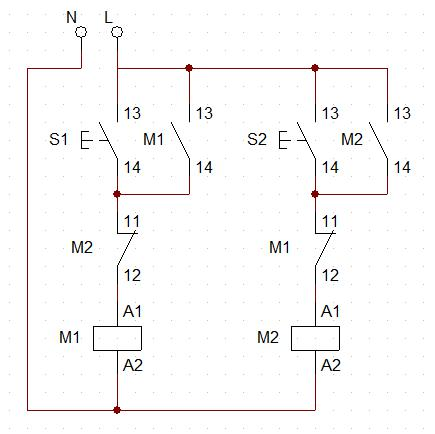
\includegraphics[width=1\linewidth]{Figuras/Ch10/fig8n3}
	\end{minipage}
	\hfill
	\begin{minipage}{0.48\linewidth}
		\centering
		
		\begin{tikzpicture}[circuit plc ladder, thick,x=1\ladderskip,y=01\ladderskip]
		
		\draw (0,0) 
		to[contact NO={info={a}}] ++(1,0) coordinate(laddercoil)
		to[contact NC={info={M\_2}}] ++(1,0) -- ++(1.5,0) 
		to[coil={info={M\_1}}] ++(1,0) coordinate(laddertopright);
		\draw (0,-1)
		to[contact NO={info={M\_1}}] ++(1,0) -- (laddercoil);
		\ladderrungend{2}
		\draw (0,0)
		to[contact NO={info={b}}] ++(1,0) coordinate(laddercoil)
		to[contact NC={info={M\_1}}] ++(1,0) -- ++(1.5,0) 
		to[coil={info={M\_2}}] ++(1,0);
		\draw (0,-1)
		to[contact NO={info={M\_2}}] ++(1,0) -- (laddercoil);
		\ladderrungend{2.1}
		
		\powerrails
		\end{tikzpicture}
	\end{minipage}

	\centering
	\bigskip
	
	Comparação entre o circuito original e seu análogo em Ladder
\end{frame}






\begin{frame}{Blocos de detecção de bordas}
	\begin{block}{Introdução}
		\begin{itemize}
			\item O Ladder conta com blocos funcionais que realizam funções úteis ao programador, desde a contagem até a detecção de bordas ou comparações matemáticas.
			\item As bordas são característica de \textbf{qualquer sinal binário}, e podem ser necessárias para o \textbf{controle rigoroso} de uma variável.
		\end{itemize}
	\end{block}

	\centering

	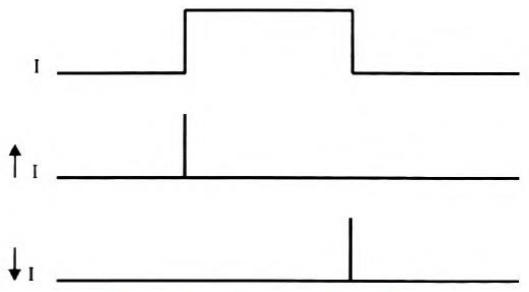
\includegraphics[width=0.7\linewidth]{Figuras/Ch10/fig7}
	
\end{frame}


\begin{frame}{Blocos de detecção de bordas}
	\begin{block}{ONS}
		\begin{itemize}
			\item O bloco ONS (\textit{One Shot}) é utilizado para detecção de bordas na mesma linha onde ficará o sinal desejado, sendo, portanto, compacto.
			\item Esse bloco detecta bordas de subida, ou seja, quando o sinal transiciona de \textbf{0 para 1}.
		\end{itemize}
	\end{block}
	
	\vspace{0.5cm}
	
	\centering
	
	\begin{tikzpicture}[circuit plc ladder, thick,x=1\ladderskip,y=01\ladderskip]
	
	\draw (0,0) 
	to[contact NO={info={a}}] ++(1.5,0) -- 
	node[midway,fill=white,draw] {ONS} node[midway, above=7pt] {aux\_1} ++(1.5,0) -- ++(2,0) 
	to[coil={info={b}, symbol=L}] ++(2,0) coordinate(laddertopright);
	\ladderrungend{2}
	
	\powerrails
	\end{tikzpicture}
	
\end{frame}


\begin{frame}{Blocos de detecção de bordas}
	\begin{block}{OSR e OSF}
		\begin{itemize}
			\item Os blocos OSR (\textit{One Shot Rising}) e OSF (\textit{One Shot Falling}) são similares ao ONS, porém, \textbf{externalizam sua saída para uma variável auxiliar}.
			\item Seus outputs são SB (\textit{Storage Bit}) e OB (\textit{Output Bit}).
			\item O SB \textbf{guarda o último valor} assumido pela entrada e aguarda uma mudança.
			\item Quando a entrada \textbf{muda de estado}, o SB se \textbf{atualiza}.
			\item Caso a borda corresponda com a função do bloco, ele \textbf{pulsará} o OB durante \textbf{um ciclo} do CLP.
		\end{itemize}
	\end{block}
\end{frame}


\begin{frame}{Blocos de detecção de bordas}
	\begin{block}{OSR}
		\begin{itemize}
			\item O bloco \textbf{OSR} detecta bordas de \textbf{subida} (0 para 1).
			\item Caso o SB indique 0 em um ciclo e então o contato ``a'' \textbf{se fechar}, SB muda para 1 e o bloco OSR \textbf{pulsará} OB por \textbf{1 ciclo}.
		\end{itemize}
	\end{block}

	\vspace{0.5cm}
	
	\centering
	
	\begin{tikzpicture}[circuit plc ladder, thick,x=1\ladderskip,y=01\ladderskip]
	
	\draw (0,0) 
	to[contact NO={info={a}}] ++(2,0) -- ++(2,0) 
	to[block={symbol=OSR,outputs={SB,OB},name=o1,minimum width=1.6cm,output sep=1.5em}] ++(1.5,0)
	to[coil={info={S\_1}}] ++(1.5,0) coordinate(laddertopright);
	\draw (o1.output 2) -- +(0.3cm,0) node[right] {O\_1};
	\ladderrungend{1.2}
	\draw (0,0)
	to[contact NO={info={O\_1}}] ++(2,0) -- ++(3,0)
	to[coil={info={b}, symbol=L}] ++(2,0);
	\ladderrungend{2}
	
	\powerrails
	\end{tikzpicture}
\end{frame}


\begin{frame}{Blocos de detecção de bordas}
	\begin{block}{OSR}
		\begin{itemize}
			\item O bloco \textbf{OSF} detecta bordas de \textbf{descida} (1 para 0).
			\item Caso o SB indique 1 em um ciclo e então o contato ``a'' \textbf{se abrir}, SB muda para 0 e o bloco OSR \textbf{pulsará} OB por \textbf{1 ciclo}.
		\end{itemize}
	\end{block}
	
	\vspace{0.5cm}
	
	\centering
	
	\begin{tikzpicture}[circuit plc ladder, thick,x=1\ladderskip,y=01\ladderskip]
	
	\draw (0,0) 
	to[contact NO={info={a}}] ++(2,0) -- ++(2,0) 
	to[block={symbol=OSF,outputs={SB,OB},name=o1,minimum width=1.6cm,output sep=1.5em}] ++(1.5,0)
	to[coil={info={S\_1}}] ++(1.5,0) coordinate(laddertopright);
	\draw (o1.output 2) -- +(0.3cm,0) node[right] {O\_1};
	\ladderrungend{1.2}
	\draw (0,0)
	to[contact NO={info={O\_1}}] ++(2,0) -- ++(3,0)
	to[coil={info={b}, symbol=L}] ++(2,0);
	\ladderrungend{2}
	
	\powerrails
	\end{tikzpicture}
\end{frame}


\begin{frame}{Blocos de detecção de bordas}
	\begin{block}{Revisão}
		01. Como poderia ser feita a detecção da borda \textbf{de subida} na expressão abaixo?
		
		\[ a\cdot\notted{b}=c \]
		
		\medskip
		
		02. Cite uma utilidade dos blocos de detecção de bordas.
		
		\bigskip
		
		03. Numa fábrica existem 3 motores que não podem funcionar juntos. Elabore um circuito em Ladder que atenda a essa especificação.
	\end{block}
\end{frame}


\begin{frame}{Bloco temporizador}
	\begin{block}{TON e TOF}
		\begin{itemize}
			\item Os blocos \textbf{temporizadores} são muito úteis para garantir o funcionamento adequado de certos equipamentos.
			\item Suponha que um motor precise de \SI{15}{\second} ligado antes de ser conectado a um mixer.
			\item Com o bloco temporizador, é possível garantir que esse intervalo seja respeitado sem grandes dificuldades.
		\end{itemize}
	\end{block}

	\centering
	
	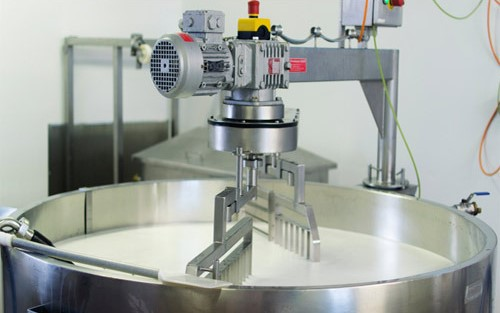
\includegraphics[height=0.45\textheight]{Figuras/Ch10/fig8}
	
\end{frame}


\begin{frame}{Bloco temporizador}
	\begin{block}{TON e TOF}
		\begin{itemize}
			\item O bloco TON \textbf{ativará} sua saída após o tempo programado.
			\item O bloco TOF \textbf{desativará} sua saída após o tempo programado.
		\end{itemize}
	\end{block}

	\medskip
	
	\centering
	
	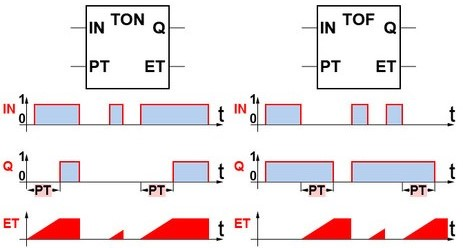
\includegraphics[height=0.6\textheight]{Figuras/Ch10/fig9}
	
\end{frame}


\begin{frame}{Bloco temporizador}
	\begin{block}{TON e TOF}
		\begin{itemize}
			\item Os blocos TON e TOF precisam de uma variável auxiliar do tipo \textbf{TIMER}.
			\item A variável TIMER possui 3 valores e 3 bits de estado.
			\item O valor PRE (\textit{Preset}) é onde informaremos \textbf{o tempo a ser contado} (em \si{\milli\second}).
			\item O valor ACC (\textit{Accumulated} - Acumulado) é onde fica registada a \textbf{contagem atual}.
			\item O valor timebase informa o \textbf{incremento de tempo}.
			\item O bit EN (\textit{Enable} - Habilitar) nos diz se a variável TIMER está \textbf{ativada no momento}, isso é, se ela \textbf{está contando}.
			\item O bit TT (\textit{Timer Timing} - Timer Contando) nos informa se o TIMER \textbf{ainda não chegou ao Preset}.
			\item O bit DN (\textit{Done} - Terminado) nos informa se o TIMER \textbf{chegou ao Preset}.
		\end{itemize}
	\end{block}
\end{frame}


\begin{frame}{Bloco temporizador}
	\begin{block}{TON}
		\begin{itemize}
			\item O TON (\textit{Timer On-Delay}) ativará sua saída DN \textbf{somente quando} ACC \textbf{igualar ou superar} o valor definido em PRE.
			\item ACC só acumula enquanto a entrada do bloco Timer for \textbf{acionada}.
		\end{itemize}
	\end{block}

	\vspace{0.5cm}
	
	\centering
	
	\begin{tikzpicture}[circuit plc ladder, thick,x=1\ladderskip,y=01\ladderskip]
	
	\draw (0,0) 
	to[contact NO={info={a}}] ++(2,0) -- ++(2,0) 
	to[block={info={T\_1},symbol=TON,inputs={IN,PRE,ACC},outputs={EN,{$ \text{TT} $},DN},name=t1,minimum width=1.6cm,output sep=1.5em,input sep=1.5em}] ++(3,0) coordinate(laddertopright);
	\draw (t1.input 2) -- +(-0.3cm,0) node[left] {1500}
		  (t1.input 3) -- +(-0.3cm,0) node[left] {0}
		  (t1.output 2) -- +(0.3cm,0)
		  (t1.output 3) -- +(0.3cm,0);
	\ladderrungend{1.5}
	\draw (0,0)
	to[contact NO={info={T\_1.DN}}] ++(2,0) -- ++(3,0)
	to[coil={info={b}, symbol=L}] ++(2,0);
	\ladderrungend{1.5}
	
	\powerrails
	\end{tikzpicture}
\end{frame}


\begin{frame}{Bloco temporizador}
	\begin{block}{TOF}
		\begin{itemize}
			\item O TOF (\textit{Timer Off-Delay}) ativará sua saída DN \textbf{enquanto} o bloco for energizado.
			\item Depois de desenergizado, sua saída \textbf{permanecerá} ativada \textbf{até} ACC \textbf{igualar ou superar} o valor definido em PRE.
		\end{itemize}
	\end{block}
	
	\vspace{0.2cm}
	
	\centering
	
	\begin{tikzpicture}[circuit plc ladder, thick,x=1\ladderskip,y=01\ladderskip]
	
	\draw (0,0) 
	to[contact NO={info={a}}] ++(2,0) -- ++(2,0) 
	to[block={info={T\_1},symbol=TOF,inputs={IN,PRE,ACC},outputs={EN,{$ \text{TT} $},DN},name=t1,minimum width=1.6cm,output sep=1.5em,input sep=1.5em}] ++(3,0) coordinate(laddertopright);
	\draw (t1.input 2) -- +(-0.3cm,0) node[left] {1500}
	(t1.input 3) -- +(-0.3cm,0) node[left] {0}
	(t1.output 2) -- +(0.3cm,0)
	(t1.output 3) -- +(0.3cm,0);
	\ladderrungend{1.5}
	\draw (0,0)
	to[contact NO={info={T\_1.DN}}] ++(2,0) -- ++(3,0)
	to[coil={info={b}, symbol=L}] ++(2,0);
	\ladderrungend{1.5}
	
	\powerrails
	\end{tikzpicture}
\end{frame}


\begin{frame}{Bloco temporizador}
	\begin{block}{RTO e RES}
		\begin{itemize}
			\item O RTO (\textit{Retentive Timer On}) é \textbf{muito similar} ao TON, executando, basicamente, a mesma função que ele.
			\item O RTO, porém, \textbf{não reseta seu ACC por conta própria}, necessitando do bloco \textbf{RES} (\textit{Reset}) para essa função.
		\end{itemize}
	\end{block}
	
%	\vspace{0.5cm}
	
	\centering
	
	\begin{tikzpicture}[circuit plc ladder, thick,x=1\ladderskip,y=1\ladderskip]
	
	\draw (0,0) 
	to[contact NO={info={a}}] ++(2,0) -- ++(2,0) 
	to[block={info={T\_1},symbol=RTO,inputs={IN,PRE,ACC},outputs={EN,{$ \text{TT} $},DN},name=t1,minimum width=1.6cm,output sep=1.5em,input sep=1.5em}] ++(3,0) coordinate(laddertopright);
	\draw (t1.input 2) -- +(-0.3cm,0) node[left] {1500}
	(t1.input 3) -- +(-0.3cm,0) node[left] {0}
	(t1.output 2) -- +(0.3cm,0)
	(t1.output 3) -- +(0.3cm,0);
	\ladderrungend{1.3}
	\draw (0,0)
	to[contact NO={info={T\_1.DN}}] ++(2,0) -- ++(3,0)
	to[coil={info={b}, symbol=L}] ++(2,0);
	\ladderrungend{0.7}
	\draw (0,0)
	to[contact NO={info={c}}] ++(2,0) -- ++(3,0) --
	node[midway,fill=white,draw] {RES} node[midway, above=7pt] {T\_1} ++(2,0);
	\ladderrungend{1}
	
	\powerrails
	\end{tikzpicture}
\end{frame}


\begin{frame}{Bloco temporizador}
	\begin{block}{Revisão}
		01. Monte os diagramas Ladder para cada uma das situações abaixo:
		
		\medskip
		
		(a) Numa fábrica, deseja-se misturar um produto durante \SI{12}{\second} usando um mixer, toda vez que a válvula de entrada do tanque do processo for \textbf{fechada}.
		
		\bigskip
		
		(b) Devido a acidentes recentes numa planta, o gerente decidiu implementar um sistema de segurança em alguns equipamentos que só permite que sejam ativados caso \textbf{dois botões permaneçam pressionados ao mesmo tempo}, só que se \textbf{qualquer um deles} ficar pressionado sozinho por mais de \SI{2}{\second}, o circuito de ligação deve se \textbf{desarmar}.
	\end{block}
\end{frame}


\begin{frame}{Bloco contador}
	\begin{block}{CTU, CTD e RES}
		\begin{itemize}
			\item Os blocos CTU (\textit{Counter Up} - Contador Progressivo) e CTD (\textit{Counter Down} - Contador Regressivo) realizam a contagem de uma variável seguindo o mesmo padrão dos Timers.
			\item Cada contador vai ser incrementado ou decrementado quando for \textbf{pulsado}.
			\item Possuem, também, 2 valores usados na contagem, PRE e ACC, que funcionam como esperado, e 1 bit de informação, DN.
			\item O CTU contará \textbf{para cima} (0, 1, 2...) e o CTD, \textbf{para baixo}, até atingir o \textbf{zero}.
			\item O CTU ativará seu bit DN quando \textbf{atingir o valor} de PRE, e o CTD ativará DN ao \textbf{atingir o zero}.
			\item Ambos só irão \textbf{resetar a contagem} usando o bloco \textbf{RES}.
		\end{itemize}
	\end{block}
\end{frame}


\begin{frame}{Bloco contador}
	\begin{block}{CTU e RES}
		\begin{itemize}
			\item O CTU contará \textbf{para cima}, sendo resetado pelo RES.
			\item O bloco ONS é importante para \textbf{garantir o pulso}.
		\end{itemize}
	\end{block}
	
%	\vspace{0.5cm}
	
	\centering
	
	\begin{tikzpicture}[circuit plc ladder, thick,x=1\ladderskip,y=1\ladderskip]
	
	\draw (0,0) 
	to[contact NO={info={a}}] ++(1.5,0) -- 
	node[midway,fill=white,draw] {ONS} node[midway, above=7pt] {aux\_1} ++(1.5,0) -- ++(1,0) 
	to[block={info={C\_1},symbol=CTU,inputs={IN,PRE,ACC},outputs={DN},name=c1,minimum width=1.6cm,output sep=1.5em,input sep=1.5em}] ++(3,0) coordinate(laddertopright);
	\draw (t1.input 2) -- +(-0.3cm,0) node[left] {3}
	(t1.input 3) -- +(-0.3cm,0) node[left] {0};
	\ladderrungend{1.3}
	\draw (0,0)
	to[contact NO={info={C\_1.DN}}] ++(2,0) -- ++(3,0)
	to[coil={info={b}, symbol=L}] ++(2,0);
	\ladderrungend{0.7}
	\draw (0,0)
	to[contact NO={info={c}}] ++(2,0) -- ++(3,0) --
	node[midway,fill=white,draw] {RES} node[midway, above=7pt] {C\_1} ++(2,0);
	\ladderrungend{1.5}
	
	\powerrails
	\end{tikzpicture}
\end{frame}


\begin{frame}{Bloco contador}
	\begin{block}{CTD e RES}
		\begin{itemize}
			\item O CTD contará para \textbf{baixo, \textbf{partindo de PRE} e sendo resetado pelo \textbf{RES}}.
		\end{itemize}
	\end{block}
	
	%	\vspace{0.5cm}
	
	\centering
	
	\begin{tikzpicture}[circuit plc ladder, thick,x=1\ladderskip,y=1\ladderskip]
	
	\draw (0,0) 
	to[contact NO={info={a}}] ++(1.5,0) -- 
	node[midway,fill=white,draw] {ONS} node[midway, above=7pt] {aux\_1} ++(1.5,0) -- ++(1,0) 
	to[block={info={C\_1},symbol=CTD,inputs={IN,PRE,ACC},outputs={DN},name=c1,minimum width=1.6cm,output sep=1.5em,input sep=1.5em}] ++(3,0) coordinate(laddertopright);
	\draw (t1.input 2) -- +(-0.3cm,0) node[left] {3}
	(t1.input 3) -- +(-0.3cm,0) node[left] {3};
	\ladderrungend{1.3}
	\draw (0,0)
	to[contact NO={info={C\_1.DN}}] ++(2,0) -- ++(3,0)
	to[coil={info={b}, symbol=L}] ++(2,0);
	\ladderrungend{0.7}
	\draw (0,0)
	to[contact NO={info={c}}] ++(2,0) -- ++(3,0) --
	node[midway,fill=white,draw] {RES} node[midway, above=7pt] {C\_1} ++(2,0);
	\ladderrungend{1.5}
	
	\powerrails
	\end{tikzpicture}
\end{frame}


\begin{frame}{Bloco contador}
	\begin{block}{Revisão}
		01. Uma linha de produção precisa contar quantos produtos são produzidos em \textbf{um dia}, com a meta de 500 por hora. Sabendo que a fábrica funciona durante \textbf{\SI{13}{\hour} ininterruptamente}, monte o diagrama Ladder para esta situação.
		
		\bigskip
		
		02. Toda vez que um operário chega na fábrica, a porta de entrada deve \textbf{permanecer aberta} por \SI{20}{\second}, e confirmar que o operário entrou através de um \textbf{sensor} embutido com contador. Monte o diagrama Ladder para esta situação.
	\end{block}
\end{frame}


%\frame{
%	\frametitle{Exercícios}
%	\begin{block}{}
%		
%	\end{block}
%}

\section*{Referências}
\frame{
	\frametitle{Referências e Exercícios Complementares}
	\begin{itemize}
		\item FRANCHI, Claiton Moro; CAMARGO, Valter Luis Arlindo de. Controladores Lógicos Programáveis - Sistemas Discretos, 1 ed. Érica, 2008.
		\item TAVARES, Leonardo; MONTEIRO, Natália Nogueira. Controladores Lógicos Programáveis, 1 ed. [s.n.], 2017.
	\end{itemize}
	%\centering{\alert{Página 546 - \textbf{Capítulo 6}}} \\
	%\centering{\alert{Lista de exercícios 01}}
}